\documentclass{article}

\usepackage{wrapfig, blindtext} % Package to generate dummy text throughout this template 

\usepackage[sc]{mathpazo} % Use the Palatino font
\usepackage[T1]{fontenc} % Use 8-bit encoding that has 256 glyphs
\linespread{1.05} % Line spacing - Palatino needs more space between lines
\usepackage{microtype} % Slightly tweak font spacing for aesthetics

\usepackage{inputenc}

\usepackage[english]{babel} % Language hyphenation and typographical rules

% \usepackage[hmarginratio=1:1,top=32mm,columnsep=20pt]{geometry} % Document margins
% \usepackage[hang, small,labelfont=bf,up,textfont=it,up]{caption} % Custom captions under/above floats in tables or figures
\usepackage{booktabs} % Horizontal rules in tables

\usepackage{enumitem} % Customized lists
% \setlist[itemize]{noitemsep} % Make itemize lists more compact

\usepackage{titling} % Customizing the title section

\usepackage[hidelinks]{hyperref} % For hyperlinks in the PDF

\usepackage{graphicx} % For pictures
\usepackage{wrapfig}

\usepackage{amsmath}
\usepackage{algorithm}
\usepackage[noend]{algpseudocode}

%------------------------------------------------------------------------------
%	TITLE SECTION
%------------------------------------------------------------------------------

\setlength{\droptitle}{-4\baselineskip} % Move the title up

\pretitle{\begin{center}\Huge\bfseries} % Article title formatting
\posttitle{\end{center}} % Article title closing formatting
\title{Solving the MST Problem with the Skewed Filter-Kruskal Algorithm} % Article title
\author{%
\textsc{Ermanno Righini}%\thanks{A thank you or further information} 
\\[1ex] % Your name
%\normalsize Università degli Studi di Milano\\ % Your institution
%\normalsize \href{mailto:ermannorighini@gmail.com}{ermannorighini@gmail.com} % Your email address
}
\date{\today} % Leave empty to omit a date

%------------------------------------------------------------------------------

\begin{document}


% Print the title
\maketitle

%------------------------------------------------------------------------------
%	ARTICLE CONTENTS
%------------------------------------------------------------------------------

\section{Introduction}

The minimum spanning tree problem consists of finding for a graph $G=(V,E)$, the minimum weight spanning tree of $G$.
The most used and successful algorithms to solve this problem are the Prim algorithm \cite{prim} and the Kruskal algorithm \cite{kruskal}.

The Kruskal algorithm has been improved over the years, first in \cite{incremental} where the authors mixed the kruskal algorithm with the idea of incremental sort. Then it was improved again in \cite{filterkruskal} where a filtering step was introduced during the sorting.

\section{Prim Algorithm}

The Prim algorithm starts with a tree consisting of a single node, then it iteratively adds to the tree the smallest edge that connects to a node not part of the partial spanning tree. When there are no edges meeting this criteria, the procedure has produced a minimum spanning tree. The only case where this doesn't work is when the input graph is not connected and a spanning tree doesn't exist. In this case the problem becomes of finding the minimum spanning forest, and the Prim algorithm can be adapted to work on this case by simply running the Prim algorithm on all nodes of the graph that are not yet part of a spanning tree.

To efficiently find the next smallest edge it is necessary to use a priority queue, like for example the Pairing Heap data structure \cite{pairing} that I used in this project.
The time complexity of the Prim algorithm is $\mathcal{O}(E + V\log V)$.

\section{Kruskal Algorithm}

Kruskal algorithm instead follows a different approach: the list of edges is sorted in increasing weight and a forest is initialized where each node represents a tree on its own. Then starting from the smallest edge, we add all the edges that connects nodes in different trees of the forest. By the end of the procedure the forest gets collapsed to a minimum spanning tree if the graph is connected or to a minimum spanning forest otherwise.

\begin{algorithm}
    \begin{algorithmic}
        \Function{Kruskal}{$V$, $E$, $T$} \Comment{With $T$ list of MST edges}
            \For{$(x, y) \in $ \Call{Sorted}{$E$}} \Comment{Sort by increasing edge weight}
                \If{\Call{Find}{$x$} = \Call{Find}{$y$}}
                    \State \Call{Union}{$x$, $y$}
                    \State $T := T \cup \{(x, y)\}$
                \EndIf
            \EndFor
        \EndFunction
    \end{algorithmic}
\end{algorithm}

For an efficient implementation of the algorithm a Disjoint Set data structure can be used which accelerate the operations of $find(x)$, which returns the root of the tree containing $x$ and $union(x, y)$ which merges the trees of $x$ and $y$ into a single tree.

The time complexity of the algorithm is $\mathcal{O}(E\log E)$.

\subsection{Disjoint Set}

The main component of the Kruskal algorithm is the Disjoint Set data structure, which implements an efficient way of representing a collection of disjoint sets of elements and perform operation on them such as:
\begin{itemize}
    \item \textproc{Find($x$)}: returns the identifier set containing $x$.
    \item \textproc{Union($x$, $y$)}: merges the two sets containing $x$ and $y$.
\end{itemize}

An efficient implementation of \textproc{Find} can use the path compression technique, which reduces the time complexity from $\mathcal{O}(n)$ to an amortized $\mathcal{O}(\alpha(n))$. Path compression consists in caching the set identifier of $x$ and every element in the path from $x$ to the representative of the set every time the $\textproc{Find}$ procedure is called.

The \textproc{Union} procedure can instead be efficiently implemented by using the union by rank variation, where the basic idea is to always add the smaller set to the bigger one when performing a union operation.

\subsection{Quick-Kruskal Algorithm}

The Quick-Kruskal algorithm variation instead of sorting the edge list before building the MST, does the two things simultaneously. It performs sorting in a similar way to QuickSort and when the partitions become too small it falls back to the classing Kruskal algorithm.

\begin{algorithm}
    \begin{algorithmic}
        \Function{QuickKruskal}{$V$, $E$, $T$}
            \If {$\lvert E \rvert < 1000$} 
                \State \Return \Call{Kruskal}{$V$, $E$, $T$}
            \EndIf
            \State $p := $ \Call{PickPivot}{$E$}
            \State $E_1, E_2 := $ \Call{Partition}{$E$, $p$}
            \State \Call{QuickKruskal}{$V$, $E_1$, $T$}
            \If {$\lvert T\rvert < \lvert V \rvert-1$}
                \State \Call{QuickKruskal}{$V$, $E_2$, $T$}
            \EndIf
        \EndFunction
    \end{algorithmic}
\end{algorithm}

With this strategy the algorithm becomes much faster for graph with randomly generated weights, since the edge list needs to be sorted only up to the last edge contained in the MST and for randomly generated graphs the MST is contained in the first $\mathcal{O}(\lvert V\rvert\log \lvert V\rvert)$ smaller edges. On the other hand this algorithm is not very robust, because if the input graph has at least one heavy edge, then the entire list needs to be sorted and the complexity falls back to the standard Kruskal algorithm.

The time complexity of the algorithm for random graphs with random edges is $\mathcal{O}(E + V \log^2 V)$

\subsection{Filter-Kruskal Algorithm}

The Filter-Kruskal variation is an improvement upon the Quick-Kruskal algorithm, where after the partition operation, the right side of the partition is filtered of any edge adjacent to two vertices in the same tree of the forest (\textproc{Find}($x$) $ = $ \textproc{Find}($y$)).

\begin{algorithm}
    \begin{algorithmic}
        \Function{FilterKruskal}{$V$, $E$, $T$}
            \If {$\lvert E \rvert < 1000$} 
                \State \Return \Call{Kruskal}{$V$, $E$, $T$}
            \EndIf
            \State $p := $ \Call{PickPivot}{$E$}
            \State $E_1, E_2 := $ \Call{Partition}{$E$, $p$}
            \State \Call{FilterKruskal}{$V$, $E_1$, $T$}
            \If {$\lvert T\rvert < \lvert V \rvert-1$}
                \State $E_f := \{(x, y) \in E_2 : $ \Call{Find}{x} $\neq$ \Call{Find}{y}$\}$ \Comment{Filter pass}
                \State \Call{FilterKruskal}{$V$, $E_f$, $T$}
            \EndIf
        \EndFunction
    \end{algorithmic}
\end{algorithm}

This simple modification of the algorithm leads to much better performance since if the graph is not very sparse, most of the edges are not part of the MST and get filtered away during the incremental sorting of the edge list, making the sorting of the remaining portion of the list easier as more edges are added to the MST.

The time complexity of the algorithm for random graphs with random edge weights is $\mathcal{O}(\lvert E\rvert + \lvert V\rvert \log \lvert V \rvert \log \frac{\lvert E \rvert}{\lvert V\rvert})$

\subsection{Skewed Filter-Kruskal Variation}

To further improve the Filter-Kruskal algorithm I made the assumption that in random graphs with random edges the MST is contained in the first $\mathcal{O}(\lvert V\rvert\log \lvert V\rvert)$ smallest edges and more generally in most graphs a good portion of the MST is contained in the smallest edges of the graph if the graph is dense enough. 

To leverage this, in the first recursion level of \textproc{FilterKruskal} I perform a skewed partitioning, where the first partition has size $k\lvert V \rvert /\log \lvert V\rvert$ where $k$ is a constant slightly bigger than $1$. And in every other recursion level I split the edge list in half. From my tests I actually found out that using a skewed partitioning method even in inner recursion levels doesn't degrade performance. I think this happens because by using a skewed partitioning I improve the branch miss-prediction rate and the edges get filtered away earlier, decreasing the cost of the sorting. On the other hand the recursion depth increases, so the two effects roughly balance each other.

\subsection{Picking a Pivot}

I tested different strategies for picking a pivot, such as:
\begin{itemize}
    \item \textbf{1 Sample Random Pivot}: Select one element randomly from the edge list and use its weight as a pivot.
    \item \textbf{3 Samples Random Pivot}: Select three elements randomly and use the median as the pivot.
    \item \textbf{$\sqrt n$ Samples Random Pivot}: Select $\sqrt n$ elements randomly and use the median as pivot.
\end{itemize}

For the \textproc{FilterKruskal} implementation I found that picking just one sample turned out to be the fastest, though this strategy introduces more variability in the execution time of the procedure, since in particular in the first recursion levels a bad pivot can worsen the performance significantly.

For the \textproc{SkewedFilterKruskal} implementation, since I need to be more precise with the pivot selection I decided to use instead the "root of $n$" approach. This produces much better pivots but at the same time it's much slower (for very dense graphs the number of pivot is close to the size of the MST). 

One way to mitigate this performance penalty is to pick a sample of size $\sqrt n$ one time at the start of the procedure and reuse the pivot from the sample at every recursion level until all the pivots in a given range have been exhausted, and then go back to a single random sample per pivot.

\section{Using Multiple Pivots}

Another approach I tried to improve the Filter-Kruskal algorithm is to use more than one pivot in the partitioning phase.

The rationale behind this idea is that if the MST edges are contained in the smallest edges of the graph then I only need to explore the first partition (which should be smaller than the one generated by the Filter-Kruskal algorithm) and I only read once the rest of the unneeded edges. In the case that instead I need to read the entire edge list the sorting is facilitated since I already partitioned the input list in many small lists. So if the constant costs introduced by adding more pivots are small I expect to see an improvement in execution times.

\subsection{Sample Sort}

The Samplesort algorithm can be thought of as a generalization of quicksort to $k$ pivots. The basic idea is that we extract a sample of elements of size $\mathcal O(k\sqrt n)$ from the input list so that we can calculate good pivots to perform the partitioning. Implementations of samplesort vary the pivot count from a few dozen to a few thousands.

In particular I decided to adopt the implementation of Super Scalar Sample Sort \cite{samplesort} where the author showed that this implementation can beat the standard C++ sorting algorithm by a sizeable margin. The algorithm is recursive and each recursion is organized in a few steps:

\begin{itemize}
    \item \textbf{Pivot Sampling} The input list is sampled to extract $k$ pivots, which are used to subdivide the elements in $k+1$ buckets.
    \item \textbf{Build Decision Tree} A binary decision tree is built on the extracted pivots, so that for every element the corresponding bucket can be found efficiently. The bucket can be calculated without any branches.
    \item \textbf{Assign Buckets} For every element we calculate the corresponding bucket and store all the bucket ids in a list.
    \item \textbf{Calculate Bucket Sizes and Prefix Sum} During the bucket assignment phase we also calculate the bucket sizes and calculate the prefix sum of the bucket sizes in order to easily find where each bucket starts in the output continuous array.
    \item \textbf{Distribute Elements} Distribute all the elements in the corresponding bucket disposed in a contiguous array.
\end{itemize}

The algorithm was adapted to the MST problem by performing a filter step before each recursion on all buckets that were not the first one. And by running kruskal instead of a sort algorithm on the base case.

\subsection{Dual Pivot QuickSort}

I also tried the partitioning scheme proposed by \cite{dualpivot} as an improvement to quicksort. The basic idea is that we use two pivots, instead of only one, so at every recursion level we partition the list in three partitions. This compared to samplesort should introduce lower constant cost for the partitioning phase of Filter-Kruskal.

\section{Graph Generation}

Another important part of the project was the generation of graphs to use as a benchmark suite for the different algorithms. I ended up focusing on three categories of graphs:

\begin{itemize}
    \item \textbf{Random Graphs with Random Edges} These are graphs where the edges are added to the graph with a certain uniform probability $p$ and where the weights are chosen randomly between a minimum and maximum weight.
    \item \textbf{Random Graphs with 1 Long Edge} These graphs are generated in the same way as the previous category with the exception that in the graph is always present at least one edge that must be contained in the MST and that is the longest among all the other edges. This property is useful to test what happens in the case where algorithms based on Kruskal are forced to scan the entire edge list.
    \item \textbf{Random 2D Geometric Graphs} In these category of graphs, vertices are points on a 2D plane, and edges between them are the euclidean distances. For each vertex only the edges to its $k$ nearest neighbors are added to the graph. This class of graphs, compared to the other two has the property of having more clusters of vertices.
\end{itemize}

\subsection{Random Sparse Graphs Generation}

One of the problems I faced during this project was to efficiently generate sparse graphs. That is why I developed an algorithm specifically for generating sparse graphs which in my tests is faster than all other methods.

The basic idea is that instead of checking for every edge if we want to include it or not into the graph, I randomly skip to the next edge that will be included in the graph by following the correct probability distribution.

First I imagine to have an enumeration of all the possible edges for a graph with $V$ vertices, where the first edge has index $0$ and the last $V-1$.

So given $p$ as the probability of any possible edge to be included in the graph, I define the probability of skipping at least $n$ edges as:
$$p_n = (1-p)^n$$ 
Because I need to \emph{not} choose an element for at least $n$ times. I now solve in function of $n$ and I obtain that:
$$n = \left\lfloor\frac{\log{p_n}}{\log{(1-p)}}\right\rfloor$$
This means that by plugging a random value in $p_n$ I can randomly calculate the skip distance to the next edge.
In order to prove that every edge $e$ has probability $p$ of being chosen we need to show that all the probabilities of all the paths that lead to choosing $e$ sum to $p$.

It is obvious that the first edge has probability $p$ of being chosen since the only way we can choose it is if we skip $0$ edges, so: 
$$C_0 = p(1-p)^0 = p$$

If we instead by any chance choose an edge $k$ it means that we either skipped all the edges before it (this has probability $p(1-p)^k$) or before picking $k$ we picked another edge $j$ where $0 \leq j < k$. 

In this case the probability is the probability of picking $j$ times the probability of skipping from $j$ to $k$, that is: $C_jp(1-p)^{k-j-1}$

Knowing that:
\begin{align*}
\sum_{j=0}^{n-1} (1-a)a^j &= (1-a)a^0 + (1-a)a^1 + \ldots + (1-a)a^{n-1}
\\ &= 1+(- a + a)+(- a^2 + a^2) + \ldots + (- a^{n-1}+ a^{n-1}) - a^n 
\\ &= 1 - a^n
\end{align*}

If we consider all edges before $k$ we get that the probability of picking $k$ is:

\begin{align*}
C_k &= p(1-p)^k + \sum_{j=0}^{k-1} C_j p(1-p)^{k-j-1}
\\ &= p(1-p)^k + \sum_{j=0}^{k-1} p^2(1-p)^{k-j-1} \tag{Assume by induction that $C_j = p$}
\\ &= p(1-p)^k + p\sum_{j=0}^{k-1} p(1-p)^{j}
\\ &= p(1-p)^k + p\sum_{j=0}^{k-1} (1-q)q^{j} \tag{With $q=(1-p)$}
\\ &= p(1-p)^k + p(1 - q^k)
\\ &= p(1-p)^k + p(1 - (1-p)^k)
\\ &= p(1-p)^k + p - p(1-p)^k
\\ &= p
\end{align*}

By using this method for the generation of graphs the complexity becomes linear in the number of generated edges, instead of linear in the number of total possible edges.

\begin{algorithm}
    \begin{algorithmic}
        \Function{GenGraph}{$N$, $p$, $E$} \Comment{$N$ number of vertices}
            \State $a:= b := 0$
            \While{True}
                \State $k := $ \Call{Random}{$0, 1$}
                \State $skip := 1 + \left\lfloor\frac{\log(k)}{\log(1-p)}\right\rfloor$
                \State $b := b + skip$
                \While{$b \geq N$}
                    \State $a := a + 1$
                    \State $b := a - n + 1$
                \EndWhile
                \If{$a \geq N-1$} \Return
                \EndIf
                \State $E := E \cup \{(a,b)\}$
            \EndWhile
        \EndFunction
    \end{algorithmic}
\end{algorithm}

In my implementation I decided to enumerate the edges of the upper triangular matrix from the adjacency matrix of the graph, so that $0 \leq a < b < N$ for any valid edge.

\subsection{Random Geometric Graphs Generation}

For the generation of geometric graphs I first randomly place all the graph vertices on a 2D area, and then for each vertex I select add the edges relative to its $k$ closest neighbors. Finding the $k$ closest neighbors has cost $\mathcal O(n\log k)$, for a total cost of $\mathcal O(n^2\log k)$ for generating the graph.

We can bring the time complexity down to $\mathcal O(kn\log k\log n)$ by organizing the vertices in a k-d tree, which is an n-dimensional generalization of a binary search tree. In a k-d tree at a given depth $d$, the points are compared along the dimension $d \bmod k$.

The construction of a balanced tree can be achieved recursively, where at each step the elements belonging to the current node are divided into two partitions of equal or similar size by finding the median element in linear time, with a total cost of $\mathcal O(n\log n)$.

The $k$-closest neighbors of a given vertex can be found in time $\mathcal O(k\log k\log n)$ by keeping track of the $k$ closest elements in a priority queue, and searching the tree while pruning the nodes that are too far.

\section{Experimental Results}

All test were performed on a Intel Core i5-6600 CPU @ 3.9GHz and all the source code is available at \url{https://github.com/righier/filter-kruskal}

\hspace{1cm}

As can be seen in \autoref{fig:rand}, the best performing algorithm in all graph types is Skewed Filter-Kruskal, even in the case of graphs with long edges, where the procedure is forced to read and filter all edges. And for the case geometric graphs, where the higher clustering coefficient introduces heavier edges into the MST.

The Filter-Kruskal variants with multiple pivots, like Samplesort Filter-Kruskal are performing worse than the standard Filter-Kruskal implementation, probably because of the too much higher constant cost of the partitioning method.

Lastly the Prim algorithm implemented with Pairing Heap performs better than the standard Filter-Kruskal algorithm for denser graphs.

\begin{figure}[htp]
    \centering
    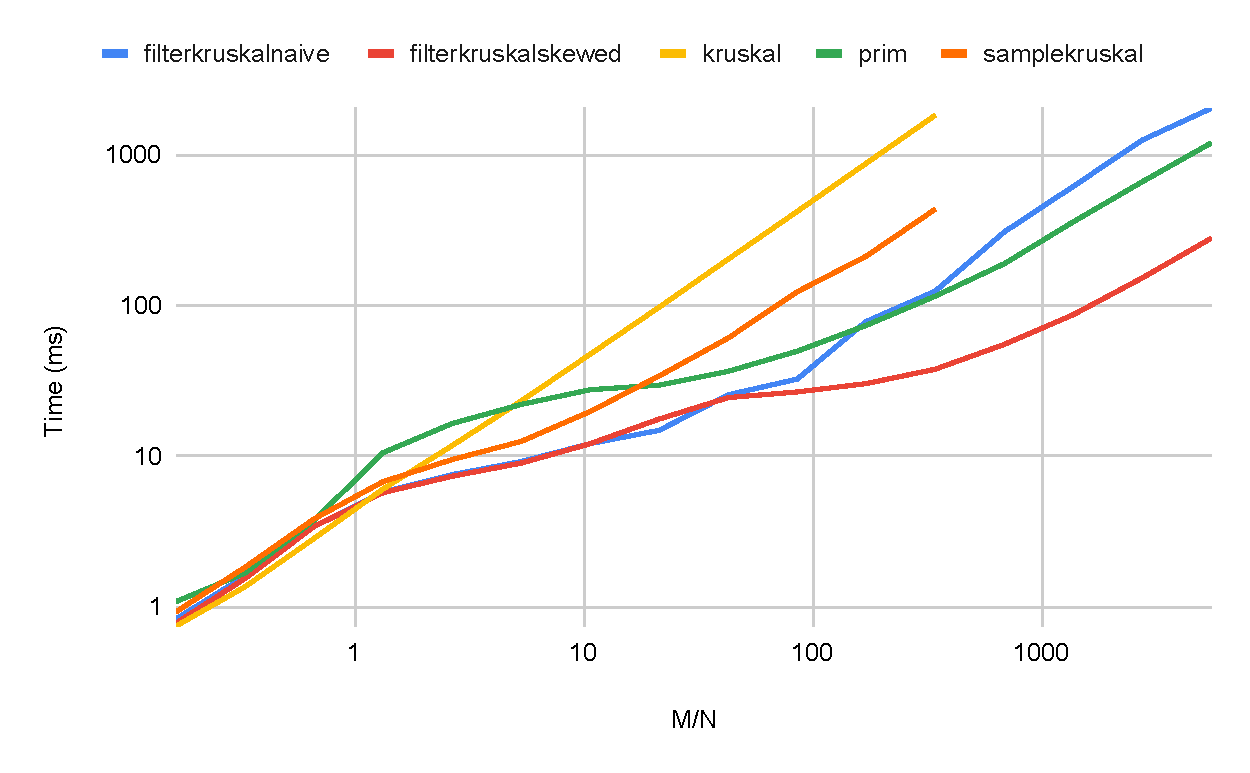
\includegraphics[width=.7\linewidth]{images/randgraph.pdf}
    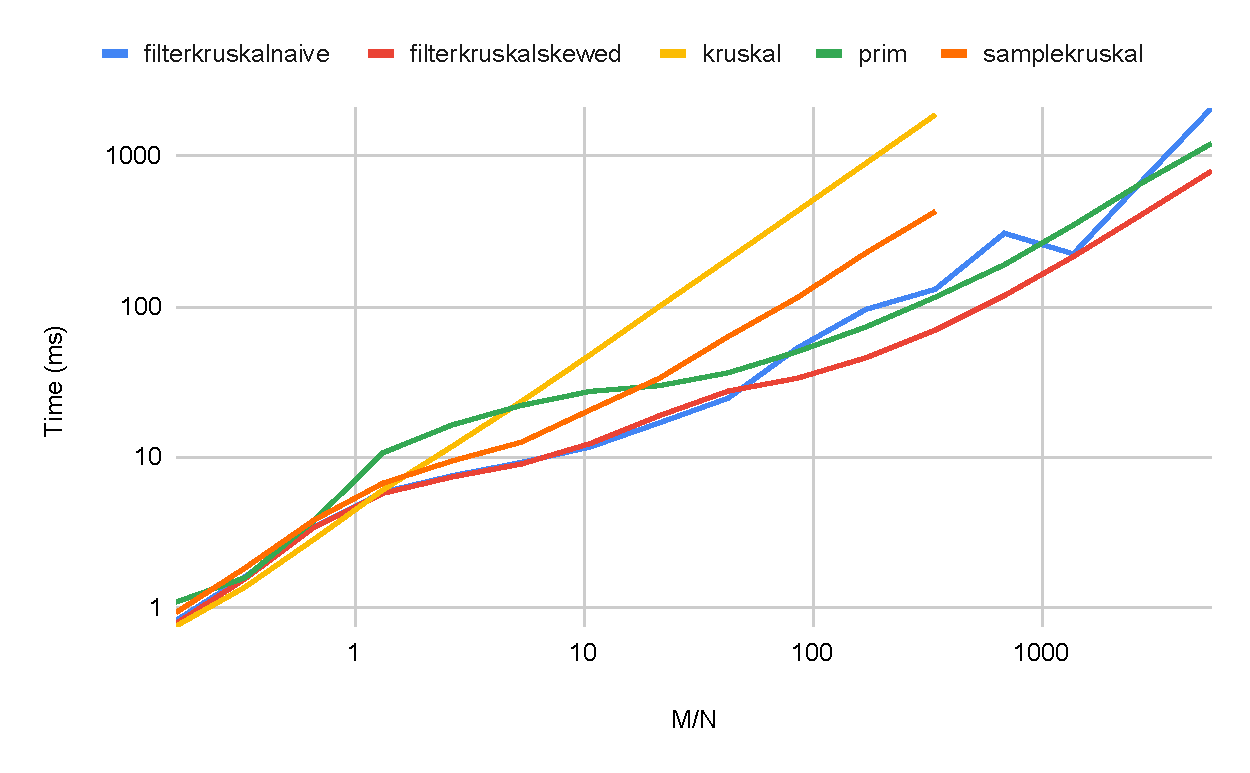
\includegraphics[width=.7\linewidth]{images/hardgraph.pdf}
    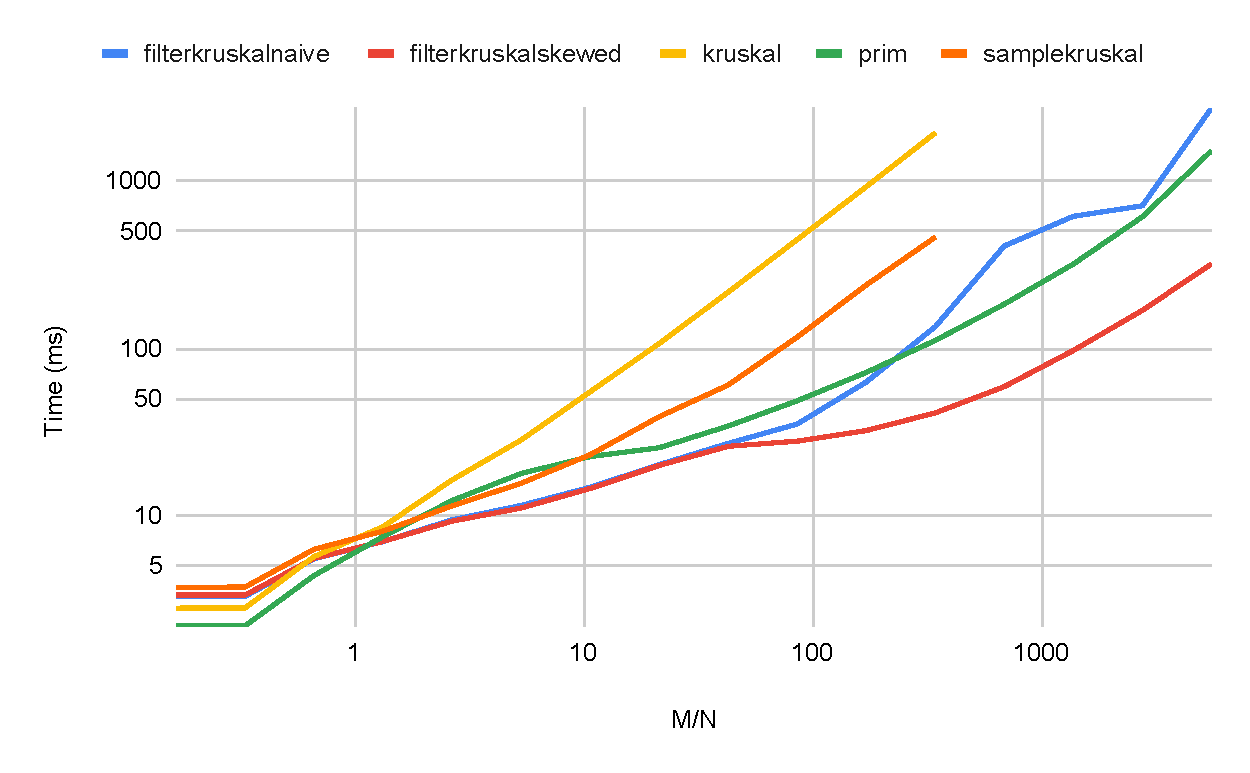
\includegraphics[width=.7\linewidth]{images/geomgraph.pdf}
    \caption{Comparison of different algorithms on different graph types. From top to bottom: 1) graphs with random weights, 2) graphs with one long edge, 3) random geometric graphs}
    \label{fig:rand}
\end{figure}

\section{Conclusions}

The results of this project didn't turn up as I expected, in particular I thought that the Filter-Kruskal variants based on multiple pivots would perform much better than they did in reality. 

One way in which these kinds of algorithms (in particular samplesort) could bring an advantage is in an eventual parallel implementation of the algorithm, since individual steps of the samplesort algorithm are good candidates for parallelization.

%----------------------------------------------------------------------------------------
%	REFERENCE LIST
%----------------------------------------------------------------------------------------

\bibliographystyle{unsrt}
\bibliography{biblio}


%----------------------------------------------------------------------------------------

\end{document}

